% =============================================================================
%  IMP302m course project report -- IEEE conference format (IEEEtran)
%  Compiles with pdfLaTeX (Overleaf default). Run twice for references.
% =============================================================================
\documentclass[conference,a4paper]{IEEEtran}
\IEEEoverridecommandlockouts

\usepackage[T5,T1]{fontenc}  % T5 only for the Vietnamese author names; T1 stays the default
\usepackage[utf8]{inputenc}
\usepackage{cite}
\usepackage{amsmath,amssymb}
\usepackage{graphicx}
\usepackage{booktabs}
\usepackage{multirow}
\usepackage{array}
\usepackage[table]{xcolor}
\usepackage{tikz}
\usetikzlibrary{arrows.meta,calc}
\usepackage{url}
\usepackage[hidelinks]{hyperref}

\definecolor{realc}{HTML}{B5471B}   % steps used only by the real-image branch
\definecolor{best}{HTML}{E3EEFB}    % highlighted (final) configuration
\definecolor{gtred}{HTML}{E34948}
\definecolor{predblue}{HTML}{2A78D6}
\newcommand{\cfg}[1]{\texttt{#1}}
\newcommand{\vn}[1]{{\fontencoding{T5}\selectfont #1}}  % Vietnamese diacritics under pdfLaTeX
\graphicspath{{figures/}}

\begin{document}

\title{Segmentation, Counting and Size Classification of Objects on a Static Background with Classical Image Processing: From Synthetic Scenes to 960 Real Photographs}

\author{
\IEEEauthorblockN{\vn{Ngô Quang Huy}}
\IEEEauthorblockA{FPT University, Vietnam\\
\texttt{ngoquanghuy2k5@gmail.com}}
\and
\IEEEauthorblockN{\vn{Nguyễn Đức Mạnh}}
\IEEEauthorblockA{FPT University, Vietnam\\
\texttt{Manhndse180326@fpt.edu.vn}}
\and
\IEEEauthorblockN{\vn{Hoàng Văn Anh}}
\IEEEauthorblockA{FPT University, Vietnam\\
\texttt{anhhvse180142@fpt.edu.vn}}
}

\maketitle

% -----------------------------------------------------------------------------
\begin{abstract}
We present a training-free, classical image-processing system that separates discrete objects (coins) from a static background, counts them, measures their geometry and classifies them into two size classes, \emph{Large} and \emph{Small}. The pipeline has four stages: gray-level preprocessing, segmentation with binary morphology, connected-component labeling with feature extraction, and rule-based classification. The core algorithms (FSHS, median and Gaussian filtering, Otsu, K-Means, erosion/dilation and two-pass labeling) are implemented from scratch in NumPy and verified to match OpenCV. The system is evaluated on four synthetic cases with pixel-exact ground truth (ideal, low contrast, noise and glare, overlapping objects) and on four real-image cases drawn from 960 smartphone photographs of the Roboflow~100 \emph{coins} dataset (ideal, low contrast, textured background, touching coins). On the synthetic cases, every object is counted and classified correctly (mask IoU $0.961$--$0.972$). On real photographs, however, the baseline counts exactly right in only $12.9\%$ of the held-out test images (F1~$=0.450$), because coins cover only about $2\%$ of the image and the background is not uniform. We therefore add a real-image branch inspired by change detection: background estimation with a large median filter, Triangle thresholding of a Lab color-difference image, border clearing, circularity-gated watershed and shape filtering. With all parameters selected on a separate development split, the final configuration reaches $65.4\%$ exact-count accuracy, a mean absolute counting error of $0.77$ objects per image and F1~$=0.940$ on the test split (480 images, 3\,386 coins), at about $65$\,ms per image on a CPU. Per-case results range from F1~$=0.977$ on ideal real scenes to $0.805$ on touching coins. We also show that linear histogram stretching does not change Otsu's segmentation, and that a correct count does not imply a correct segmentation.
\end{abstract}

\begin{IEEEkeywords}
image segmentation, Otsu thresholding, mathematical morphology, connected-component labeling, watershed, background subtraction, object counting
\end{IEEEkeywords}

% =============================================================================
\section{Introduction}
% =============================================================================
Counting and size-grading products laid out on a flat surface is a recurring task in automated optical inspection (AOI), agriculture (grading seeds and beans) and pharmaceuticals (counting tablets). Done by hand, it is slow, error-prone and inconsistent. This project builds a computer-vision system that automates the chain \emph{acquisition $\rightarrow$ preprocessing $\rightarrow$ segmentation $\rightarrow$ measurement and classification}, and in doing so exercises the core material of the IMP302m course~\cite{bovik2005handbook,gonzalez2018dip}.

We deliberately choose \emph{classical} image processing. It needs no labeled training data, runs in real time on a CPU, and every step can be explained by an explicit formula. The price is a dependence on scene assumptions: a roughly uniform background and a top-down view. The goal of this report is therefore not only to describe a pipeline, but to \emph{measure how far those assumptions hold} when moving from controlled synthetic scenes to real photographs.

\textbf{Contributions.}
\begin{itemize}
\item A complete four-stage pipeline whose core algorithms are implemented from scratch and verified against OpenCV (Section~\ref{sec:verify}).
\item Four synthetic test cases with pixel-exact ground truth, each isolating one difficulty and therefore one module (FSHS, morphology, watershed).
\item Four matching \emph{real-image} cases defined automatically from 960 annotated photographs, evaluated with a development/test protocol and object-level metrics. A dedicated real-image branch raises exact-count accuracy on the test split from $12.9\%$ to $65.4\%$.
\item Three verified observations: (i) linear FSHS has no effect on Otsu; (ii) two-cluster K-Means on gray levels converges to the same threshold as Otsu on the synthetic images; (iii) a correct count does not guarantee a correct segmentation.
\end{itemize}

% =============================================================================
\section{Background and Related Work}
% =============================================================================
\subsection{Thresholding}
Otsu's method~\cite{otsu1979} selects the threshold that maximizes the between-class variance of the histogram and is the standard choice for bimodal histograms. The iterative Ridler--Calvard scheme~\cite{ridler1978}, like K-Means~\cite{macqueen1967} with $k=2$ on gray levels, converges to the midpoint of the two class means. When objects occupy only a tiny fraction of the image, the histogram is essentially unimodal; the Triangle method of Zack \emph{et al.}~\cite{zack1977} is then usually more appropriate. Sezgin and Sankur~\cite{sezgin2004} survey and benchmark more than forty thresholding techniques.

\subsection{Morphology and Region Labeling}
Erosion, dilation, opening and closing~\cite{serra1982} clean binary masks. Two-pass labeling with an equivalence table~\cite{rosenfeld1966} turns a set of foreground pixels into connected regions, which is the basis for counting and measuring individual objects.

\subsection{Separating Touching Objects}
A binary image loses the boundary between two touching objects of the same color, the ``risk of oversimplification'' of binary images~\cite{bovik2005handbook}. Watershed segmentation~\cite{vincent1991,meyer1994} on the distance map, seeded at local maxima, is the classical remedy.

\subsection{Change Detection}
In video, change detection compares the current frame with a reference (background) frame to locate moving regions~\cite{radke2005}. Our real-image branch applies the same idea to a still image: the background is estimated from the image itself, and pixels that differ from it are flagged.

\subsection{Deep Learning}
Detectors such as Faster R-CNN~\cite{ren2015}, YOLO~\cite{redmon2016} and DETR~\cite{carion2020}, and Transformer backbones such as ViT~\cite{dosovitskiy2021}, achieve high accuracy on cluttered scenes. However, they require thousands of labeled images, GPU training and offer limited interpretability. Roboflow~100~\cite{ciaglia2022rf100} is a multi-domain detection benchmark built for such models; we use its \emph{coins} subset as real data. We do \emph{not} train a deep model; a qualitative comparison is given in Section~\ref{sec:discussion}.

% =============================================================================
\section{Method}\label{sec:method}
% =============================================================================
\begin{figure*}[!t]
\centering
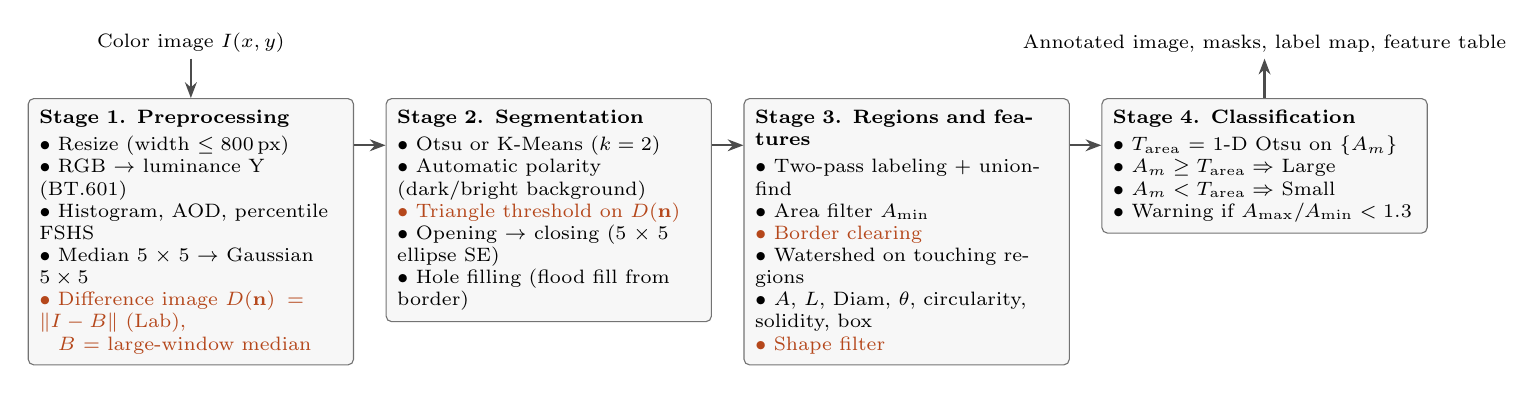
\begin{tikzpicture}[
  stage/.style={draw=black!55, rounded corners=2pt, fill=black!3, align=left,
                text width=3.85cm, inner sep=4pt, font=\scriptsize},
  io/.style={font=\scriptsize, align=center, inner sep=2pt},
  arr/.style={-{Stealth[length=2mm]}, thick, black!70}]
\node[stage, anchor=north west] (s1) at (0,0) {%
  \textbf{Stage 1. Preprocessing}\\[2pt]
  $\bullet$ Resize (width $\leq 800$\,px)\\
  $\bullet$ RGB $\rightarrow$ luminance Y (BT.601)\\
  $\bullet$ Histogram, AOD, percentile FSHS\\
  $\bullet$ Median $5\times5$ $\rightarrow$ Gaussian $5\times5$\\
  \textcolor{realc}{$\bullet$ Difference image $D(\mathbf{n})=\lVert I-B\rVert$ (Lab),}\\
  \textcolor{realc}{\phantom{$\bullet$} $B$ = large-window median}};
\node[stage, anchor=north west] (s2) at ($(s1.north east)+(4mm,0)$) {%
  \textbf{Stage 2. Segmentation}\\[2pt]
  $\bullet$ Otsu or K-Means ($k=2$)\\
  $\bullet$ Automatic polarity (dark/bright background)\\
  \textcolor{realc}{$\bullet$ Triangle threshold on $D(\mathbf{n})$}\\
  $\bullet$ Opening $\rightarrow$ closing ($5\times5$ ellipse SE)\\
  $\bullet$ Hole filling (flood fill from border)};
\node[stage, anchor=north west] (s3) at ($(s2.north east)+(4mm,0)$) {%
  \textbf{Stage 3. Regions and features}\\[2pt]
  $\bullet$ Two-pass labeling + union-find\\
  $\bullet$ Area filter $A_{\min}$\\
  \textcolor{realc}{$\bullet$ Border clearing}\\
  $\bullet$ Watershed on touching regions\\
  $\bullet$ $A$, $L$, $\mathrm{Diam}$, $\theta$, circularity, solidity, box\\
  \textcolor{realc}{$\bullet$ Shape filter}};
\node[stage, anchor=north west] (s4) at ($(s3.north east)+(4mm,0)$) {%
  \textbf{Stage 4. Classification}\\[2pt]
  $\bullet$ $T_{\text{area}}$ = 1-D Otsu on $\{A_m\}$\\
  $\bullet$ $A_m \geq T_{\text{area}} \Rightarrow$ Large\\
  $\bullet$ $A_m < T_{\text{area}} \Rightarrow$ Small\\
  $\bullet$ Warning if $A_{\max}/A_{\min} < 1.3$};
\node[io, anchor=south] (in) at ($(s1.north)+(0,5mm)$) {Color image $I(x,y)$};
\node[io, anchor=south] (out) at ($(s4.north)+(0,5mm)$) {Annotated image, masks, label map, feature table};
\draw[arr] (in.south) -- (s1.north);
\draw[arr] (s4.north) -- (out.south);
\draw[arr] ($(s1.north east)+(0,-6mm)$) -- ($(s2.north west)+(0,-6mm)$);
\draw[arr] ($(s2.north east)+(0,-6mm)$) -- ($(s3.north west)+(0,-6mm)$);
\draw[arr] ($(s3.north east)+(0,-6mm)$) -- ($(s4.north west)+(0,-6mm)$);
\end{tikzpicture}
\caption{The four-stage pipeline. Steps in \textcolor{realc}{orange} are enabled only in the real-image branch (\cfg{-{}-preset real}, Section~\ref{sec:realbranch}); all other steps are shared by both branches.}
\label{fig:pipeline}
\end{figure*}

Fig.~\ref{fig:pipeline} summarizes the system. Let $f(\mathbf{n})$, $\mathbf{n}=(n_1,n_2)$, be an $M\times N$ gray image with $K=256$ levels, $H_f(k)$ its histogram and $p(k)=H_f(k)/MN$.

\subsection{Stage 1 -- Gray-Level Preprocessing}
Images wider than 800\,px are downscaled with area interpolation; nearest-neighbor interpolation $g(\mathbf{n})=f\{\mathrm{INT}[a_1+0.5],\mathrm{INT}[a_2+0.5]\}$ is also implemented for comparison with the course material. The gray image is the luminance
\begin{equation}
f = 0.299R + 0.587G + 0.114B .
\end{equation}
Brightness is summarized by the average optical density $\mathrm{AOD}(f)=\frac{1}{MN}\sum_k k\,H_f(k)$. The full-scale histogram stretch (FSHS) is
\begin{equation}
g(\mathbf{n}) = \frac{K-1}{B-A}\,\bigl[f(\mathbf{n})-A\bigr],
\label{eq:fshs}
\end{equation}
where $A$ and $B$ are the $0.5\%$ and $99.5\%$ percentiles rather than the minimum and maximum, so that a few outliers (dust, glare) cannot disable the stretch. For denoising we apply a $5\times5$ median filter \emph{first}, to remove impulse noise, and a $5\times5$ Gaussian ($\sigma=1$) second. In the reverse order the Gaussian would smear each impulse over its neighborhood.

\subsection{Stage 2 -- Segmentation and Morphology}
\textbf{Otsu.} For a threshold $t$, the classes $C_0=\{0,\dots,t\}$ and $C_1=\{t+1,\dots,K-1\}$ have weights $\omega_0,\omega_1$ and means $\mu_0,\mu_1$. The optimal threshold is
\begin{equation}
T^{*}=\arg\max_{t}\ \omega_0(t)\,\omega_1(t)\,\bigl[\mu_0(t)-\mu_1(t)\bigr]^2 .
\label{eq:otsu}
\end{equation}

\textbf{K-Means ($k=2$).} We minimize $\sum_i\sum_{z\in C_i}\lVert z-m_i\rVert^2$ with the four steps of initialization, assignment, center update and convergence test ($E\le0.2$). Because all pixels with the same gray level fall into the same cluster, we cluster the 256 gray levels weighted by $H(k)$; this gives \emph{exactly} the same result as clustering all $MN$ pixels, at a fraction of the cost. Centers are initialized deterministically at the minimum and maximum gray level.

\textbf{Polarity.} The image border is almost always background. If most pixels in a border strip ($2\%$ of the short side) belong to the bright class, objects are the \emph{dark} class and the mask is inverted. This fixes a flaw in the original specification, which always took the bright class as foreground and therefore inverted the mask for coins on white paper.

\textbf{Morphology.} With a $5\times5$ elliptical structuring element $S$, opening $b\circ S=(b\ominus S)\oplus S$ removes isolated specks and closing $b\bullet S=(b\oplus S)\ominus S$ seals small gaps. Glare spots larger than $S$ cannot be closed, so we add \emph{hole filling}: the background is flood-filled from the image border, and every background pixel not reached is a hole inside an object.

\subsection{Stage 3 -- Labeling, Splitting and Features}
Two-pass labeling~\cite{rosenfeld1966} is implemented with a union-find equivalence table (4-connectivity); the first pass visits only foreground pixels in raster order. Regions smaller than $A_{\min}=\max(100,\ 0.0003\,MN)$ are discarded.

\textbf{Watershed.} A region is suspected to contain touching objects when its solidity $A/A_{\text{hull}}$ is below $0.94$, since the contact point creates a concavity. On its Euclidean distance map, local maxima (within a window of about $0.5\,d_{\max}$ and with value $\ge0.4\,d_{\max}$) seed a watershed~\cite{vincent1991}.

\textbf{Features.} For each region $R_m$ we compute the area $A_m=|R_m|$, the centroid $(\bar x_m,\bar y_m)$, the perimeter $L_m=\sum\Delta L$ along the closed contour with $\Delta L=\sqrt{\Delta x^2+\Delta y^2}$, the diameter $\mathrm{Diam}_m=\max_{p_i,p_j\in B_m}\lVert p_i-p_j\rVert$ (evaluated on the convex hull), the major-axis angle $\theta_m$, the circularity $4\pi A_m/L_m^2$, the solidity and the bounding box.

\subsection{Stage 4 -- Classification}
The original specification used the mean area $\bar A$ as the decision threshold. This threshold is biased whenever the numbers of large and small objects differ, or when a merged blob is present. We instead apply \emph{one-dimensional Otsu} to the sorted areas, choosing the split that maximizes $\omega_0\omega_1(\mu_0-\mu_1)^2$ as in~\eqref{eq:otsu}; the mean rule is kept as a baseline. When $A_{\max}/A_{\min}<1.3$ the system reports a single size group instead of splitting arbitrarily.

\subsection{Real-Image Branch}\label{sec:realbranch}
In real photographs, coins cover only $2.1\%$ of the image on average, while the background shows illumination gradients, table edges and wood grain. The histogram is dominated by the background, so global Otsu separates ``bright vs.\ dark background'' instead of ``coin vs.\ background'' (Fig.~\ref{fig:realgrid}, second column). We add five steps:
\begin{enumerate}
\item \textbf{Background difference.} The background $B$ is estimated with a large median filter (window $0.15\times$ the short side, computed at $1/4$ resolution). The median removes anything smaller than about $0.8$ of the window but keeps slow illumination changes. We then compute
\begin{equation}
D(\mathbf{n})=\bigl\lVert I_{\text{Lab}}(\mathbf{n})-B(\mathbf{n})\bigr\rVert_2 .
\label{eq:diff}
\end{equation}
Objects brighter \emph{or} darker than the background both yield large $D$, so no polarity decision is needed. The Lab space captures gold coins on a green mat even when their luminance matches the background.
\item \textbf{Triangle threshold}~\cite{zack1977} on $D$. A line is drawn from the histogram peak to the farthest non-empty gray level; the threshold is the level with the largest perpendicular distance to that line.
\item \textbf{Border clearing.} The specification requires objects to lie fully inside the frame, so any region touching the border is background (table edges, dark corners).
\item \textbf{Circularity-gated watershed.} Only regions with circularity $\ge0.35$ are split. Two touching coins have a circularity of about $0.5$, while table-edge strips fall below $0.3$; without this gate, the watershed chops strips into many round false positives.
\item \textbf{Shape filter.} Regions are kept only if circularity $\ge0.6$, area $\le5\%$ of the image and area $\ge0.25\times$ the median area of the remaining regions.
\end{enumerate}

% =============================================================================
\section{Experimental Setup}
% =============================================================================
\subsection{Synthetic Cases}
Four $1600\times1067$ images simulate gold (large) and silver (small) coins with drop shadows, rims, embossed patterns and JPEG compression. Each has six coins (three large, three small) and a pixel-exact ground-truth mask. Each case targets one module (Fig.~\ref{fig:synthgrid}):
\begin{itemize}
\item \textbf{Case 1 -- Ideal}: white paper, uniform lighting (baseline).
\item \textbf{Case 2 -- Low contrast}: underexposed, gray levels compressed into $[30,100]$ (FSHS).
\item \textbf{Case 3 -- Noise and glare}: dust specks, hairs, $2\%$ salt-and-pepper noise, Gaussian noise and specular glare on every coin (median filter, morphology, hole filling, area filter).
\item \textbf{Case 4 -- Overlapping}: two small coins overlap slightly (watershed).
\end{itemize}

\subsection{Real Data and Real Cases}
We use the Roboflow~100 \emph{coins} dataset~\cite{ciaglia2022rf100} (CC~BY~4.0): smartphone photographs on several backgrounds (wood, gray desks, green mats, yellow paper), resized by the publisher to $640\times640$. From its original test split (1\,599 images) we keep the \textbf{960 images that contain only coins}, with 3--9 coins each (mean $7.1$). They are split at random into a \textbf{development} set (480 images, 3\,422 coins) and a \textbf{test} set (480 images, 3\,386 coins). \emph{All design choices and parameters are selected on the development set}; the test set is run once with the chosen configurations. The annotations contain a single ``coin'' class with no size label, so on real data we evaluate counting and localization only.

To mirror the four synthetic cases, each real image is assigned to exactly one \emph{real case} using only the ground-truth boxes and image statistics, never the output of our method. The rules are applied in priority order R4 $>$ R3 $>$ R2 $>$ R1 (Table~\ref{tab:realcases}):
\begin{itemize}
\item \textbf{R4 -- Touching coins}: at least one pair of coins (circles inscribed in the boxes) touches or overlaps within 3\,px. Mirrors Case~4.
\item \textbf{R3 -- Textured background}: background roughness, i.e., the standard deviation of the high-pass gray image ($f-G_{\sigma=2}*f$) outside the coins, is in the top $30\%$ (wood grain, mat speckle). Mirrors Case~3.
\item \textbf{R2 -- Low contrast}: the median Lab color difference between each coin and a ring of surrounding background is in the bottom $30\%$. Mirrors Case~2.
\item \textbf{R1 -- Ideal}: all remaining images. Mirrors Case~1.
\end{itemize}
Percentile thresholds are computed over all 960 images.

\begin{table}[!t]
\centering
\caption{Real cases (rules applied in priority R4 $>$ R3 $>$ R2 $>$ R1). ``All'' and ``Test'' count images; ``Coins'' is for the test subset.}
\label{tab:realcases}
\footnotesize
\setlength{\tabcolsep}{3pt}
\begin{tabular}{@{}llrrr@{}}
\toprule
Case & Rule & All & Test & Coins\\
\midrule
R1 Ideal & otherwise & 477 & 232 & 1\,745\\
R2 Low contrast & coin--ring $\Delta E_{\text{Lab}} \le 48.7$ (P30) & 161 & 88 & 599\\
R3 Textured & roughness $\ge 3.74$ (P70) & 275 & 132 & 847\\
R4 Touching & a coin pair within 3\,px & 47 & 28 & 195\\
\midrule
Total & & 960 & 480 & 3\,386\\
\bottomrule
\end{tabular}
\end{table}

\subsection{Metrics}
\textbf{Counting:} exact-count accuracy (fraction of images with $\hat N_i=N_i$), the fraction within $\pm1$, and $\mathrm{MAE}=\frac{1}{|\mathcal{I}|}\sum_{i}|\hat N_i-N_i|$.

\textbf{Object level:} a prediction is a true positive (TP) if its centroid lies inside a not-yet-matched ground-truth box. Matching is one-to-one and greedy in the distance to the box center. Unmatched predictions are false positives (FP) and unmatched boxes are false negatives (FN). We report $P=\frac{TP}{TP+FP}$, $R=\frac{TP}{TP+FN}$ and $F_1=\frac{2PR}{P+R}$.

\textbf{Segmentation} (synthetic only): IoU between the predicted and ground-truth masks.

\subsection{Implementation}
The system is written in Python~3.14 with NumPy~2.5~\cite{harris2020numpy}, OpenCV~5.0~\cite{bradski2000opencv} and scikit-image~0.26 (watershed)~\cite{vanderwalt2014}. It has two interchangeable \emph{backends}: \cfg{numpy}, our own implementations, and \cfg{opencv}, library calls. All timings are single-threaded on an Intel Core i7-12700H CPU with 16\,GB of RAM. The source code, the synthetic data generator and scripts that regenerate every table and figure accompany this report.

% =============================================================================
\section{Results}
% =============================================================================
\subsection{Verification of the Own Implementation}\label{sec:verify}
Table~\ref{tab:verify} compares each hand-written algorithm with its OpenCV counterpart on the Case~3 image ($800\times534$). Median filtering, Otsu, erosion, dilation and labeling (both 4- and 8-connectivity) agree \emph{exactly}. The Gaussian filter differs by at most one gray level because OpenCV uses fixed-point rounding. At pipeline level, both backends give identical counts and F1 on real images (Section~\ref{sec:timing}).

\begin{table}[!t]
\centering
\caption{Own implementation (NumPy) vs.\ OpenCV; times in ms}
\label{tab:verify}
\footnotesize
\setlength{\tabcolsep}{4pt}
\begin{tabular}{@{}llrr@{}}
\toprule
Algorithm & Agreement & NumPy & OpenCV\\
\midrule
Median $5\times5$ & max.\ diff.\ 0 levels & 98.9 & 0.50\\
Gaussian $5\times5$ & max.\ diff.\ 1 level & 20.9 & 0.13\\
Otsu & $T^{*}=186$ in both & 1.46 & 1.65\\
Erosion & identical & 0.64 & 0.10\\
Dilation & identical & 0.55 & 0.10\\
Labeling, 4-conn. & same partition (35) & 22.3 & 1.00\\
Labeling, 8-conn. & same partition (35) & 27.4 & 0.80\\
\bottomrule
\end{tabular}
\end{table}

% -----------------------------------------------------------------------------
\subsection{Synthetic Cases}
\begin{figure*}[!t]
\centering
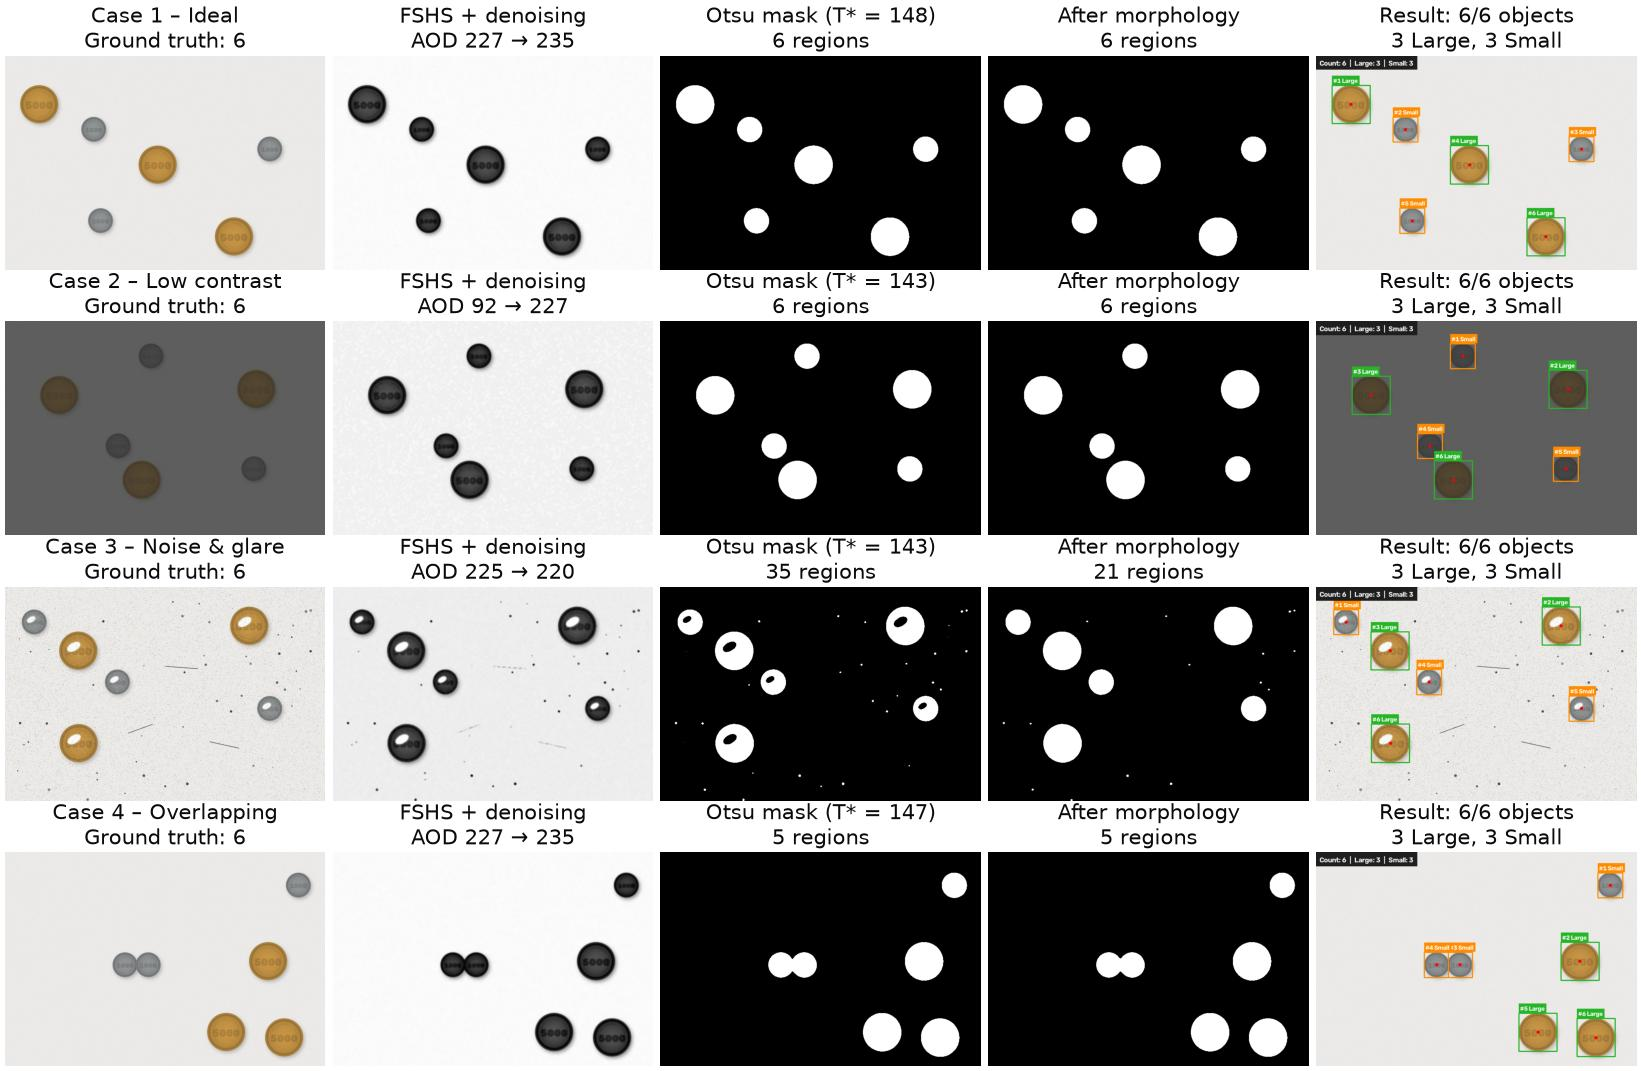
\includegraphics[width=\textwidth]{synth_grid.jpg}
\caption{The four synthetic cases (rows) through the pipeline (columns): input, FSHS with denoising, Otsu mask, mask after morphology and hole filling, and the final result with bounding boxes, centroids, IDs and size classes (green: Large, orange: Small).}
\label{fig:synthgrid}
\end{figure*}

\begin{table}[!t]
\centering
\caption{Results on the synthetic cases (default configuration: Otsu on gray). ``Raw'': regions right after thresholding; ``Morph.'': after morphology and hole filling (before the area filter); ``WS'': extra regions created by watershed.}
\label{tab:synth}
\scriptsize
\setlength{\tabcolsep}{2.4pt}
\begin{tabular}{@{}lcccccccc@{}}
\toprule
Case & AOD in/out & $T^{*}$ & Raw & Morph. & WS & Count & L/S & IoU\\
\midrule
1 Ideal & 227/235 & 148 & 6 & 6 & 0 & \textbf{6/6} & 3/3 & 0.972\\
2 Low contrast & 92/227 & 143 & 6 & 6 & 0 & \textbf{6/6} & 3/3 & 0.971\\
3 Noise/glare & 225/220 & 143 & 35 & 21 & 0 & \textbf{6/6} & 3/3 & 0.961\\
4 Overlapping & 227/235 & 147 & 5 & 5 & 1 & \textbf{6/6} & 3/3 & 0.972\\
\quad 4, no WS & 227/235 & 147 & 5 & 5 & -- & 5/6 & 4/1 & 0.972\\
\bottomrule
\end{tabular}
\end{table}

\begin{figure}[!t]
\centering
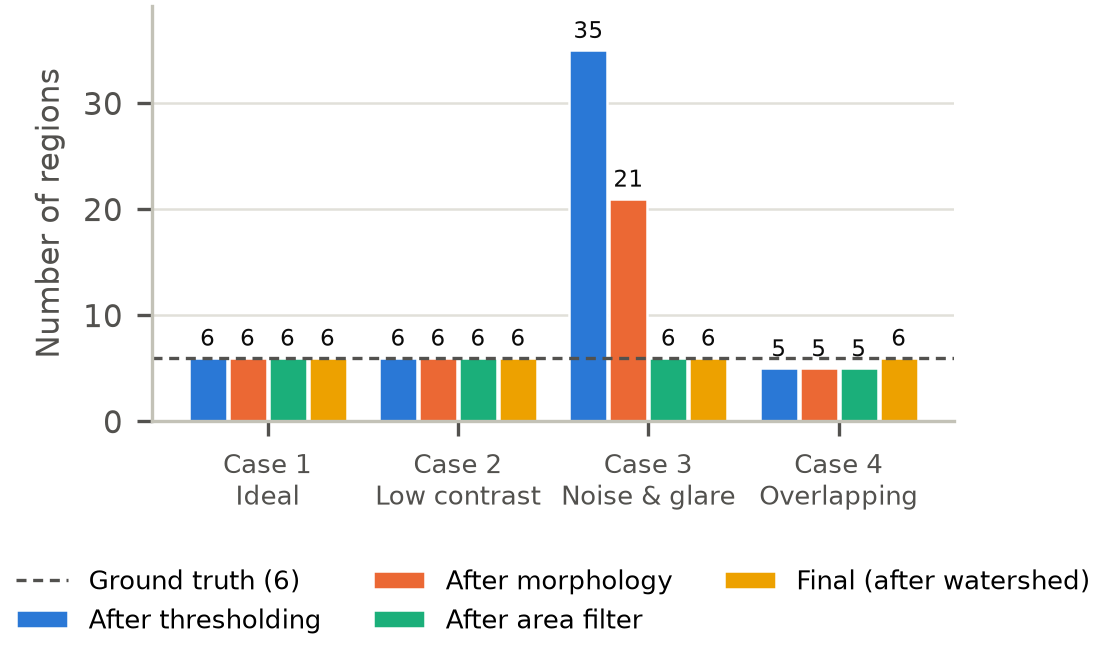
\includegraphics[width=\columnwidth]{chart_synth_regions.png}
\caption{Number of regions after each stage for the synthetic cases. Case~3: morphology removes 14 of the 29 spurious regions and the area filter removes the rest. Case~4: watershed turns 5 regions into the correct 6.}
\label{fig:synthregions}
\end{figure}

Table~\ref{tab:synth}, Fig.~\ref{fig:synthgrid} and Fig.~\ref{fig:synthregions} show that every module does its job:

\textbf{Case 1 -- Ideal.} The histogram is clearly bimodal; Otsu selects $T^{*}=148$ and every stage already has six regions. All coins are counted and classified correctly (IoU $0.972$).

\textbf{Case 2 -- Low contrast.} FSHS stretches $[A,B]=[62,96]$ to the full range and raises the AOD from $92.3$ to $227.2$ (Fig.~\ref{fig:hist}). The result is correct, but Fig.~\ref{fig:fshs} shows \emph{why}: FSHS matters only for a \emph{fixed} threshold. With $T=128$, the original image ($[30,100]$) produces an all-foreground mask, while the stretched image is segmented correctly (IoU between the two masks: $0.072$). With Otsu, the threshold moves from $80$ to $135$ but the mask is \emph{identical} (IoU $=1.000$).

\textbf{Case 3 -- Noise and glare.} Thresholding yields 35 regions (dust, hairs) and every coin has a black hole caused by glare. Opening removes small specks, closing seals gaps and hole filling closes glare holes larger than the SE (21 regions left, Fig.~\ref{fig:morph}). The area filter removes the remaining dust, leaving exactly six coins. This requires \emph{all three} defenses: median filter, morphology and area filter.

\textbf{Case 4 -- Overlapping.} Without watershed, the two small coins form one region that is counted once and classified as Large, giving 5 objects (4 Large, 1 Small). This is exactly the limitation predicted by the specification. With watershed, the result is correct (Fig.~\ref{fig:case4}).

\textbf{Otsu vs.\ K-Means.} On all four synthetic images, two-cluster K-Means converges to the \emph{same} threshold as Otsu ($148$, $143$, $143$, $147$), so the masks coincide (IoU $=1.000$).

\begin{figure}[!t]
\centering
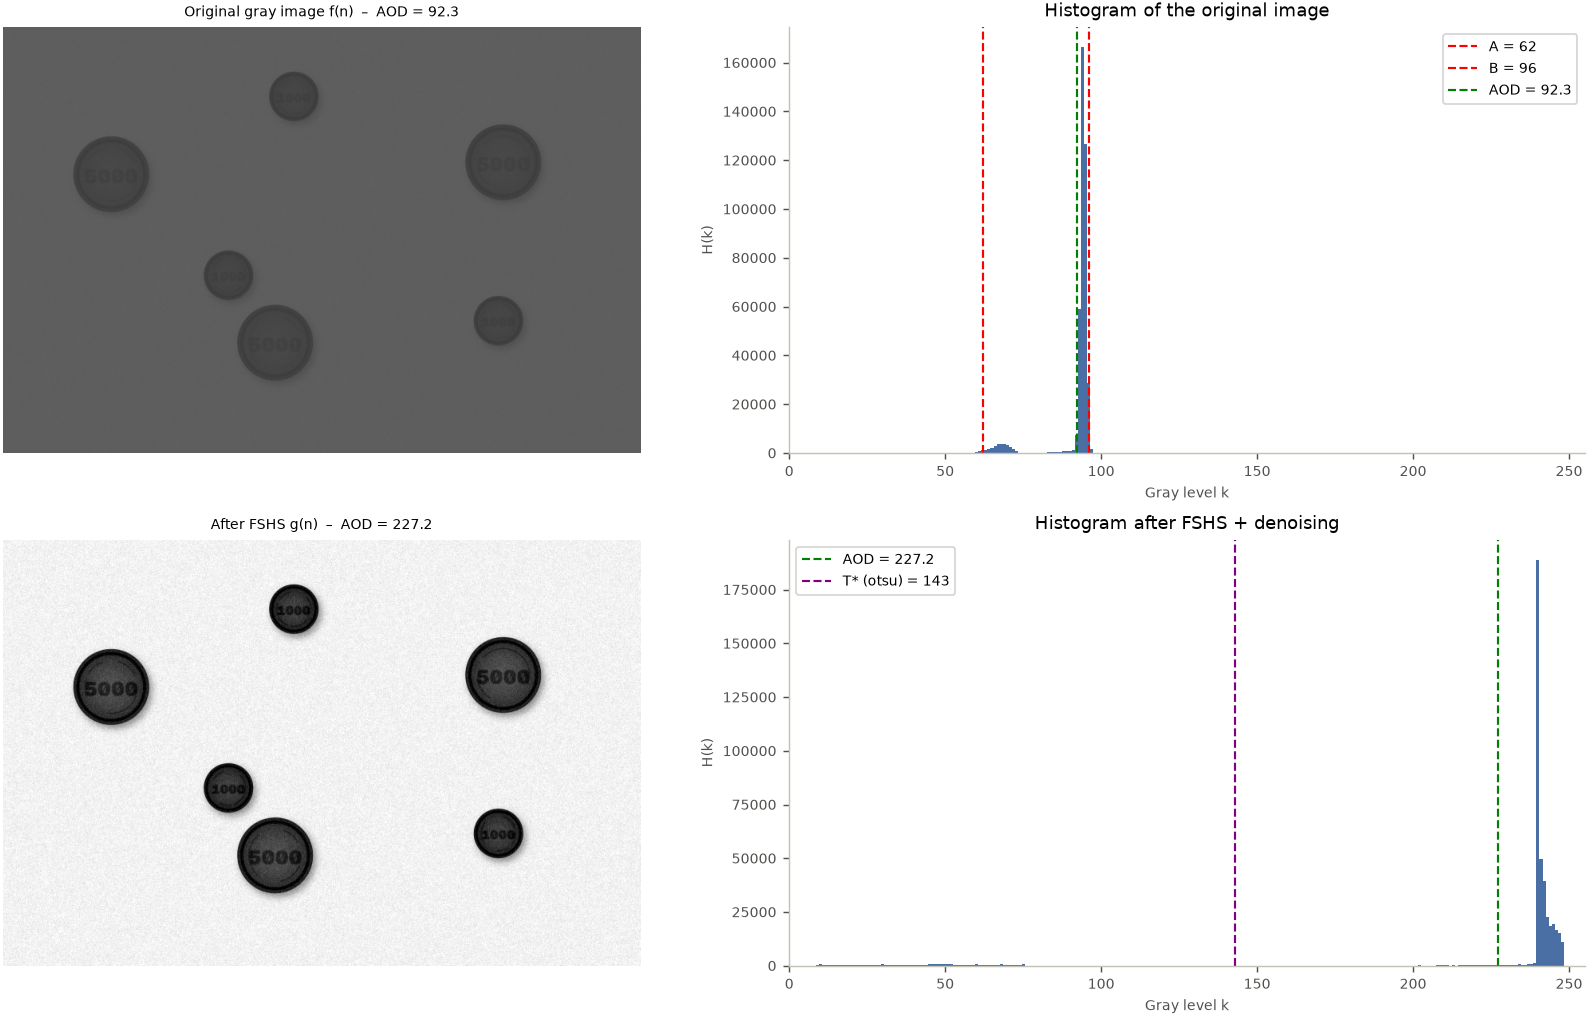
\includegraphics[width=\columnwidth]{case2_histogram.png}
\caption{Case~2: gray image and histogram before and after FSHS. The gray range $[A,B]=[62,96]$ is stretched to the full scale; the AOD rises from $92.3$ to $227.2$.}
\label{fig:hist}
\end{figure}

\begin{figure*}[!t]
\centering
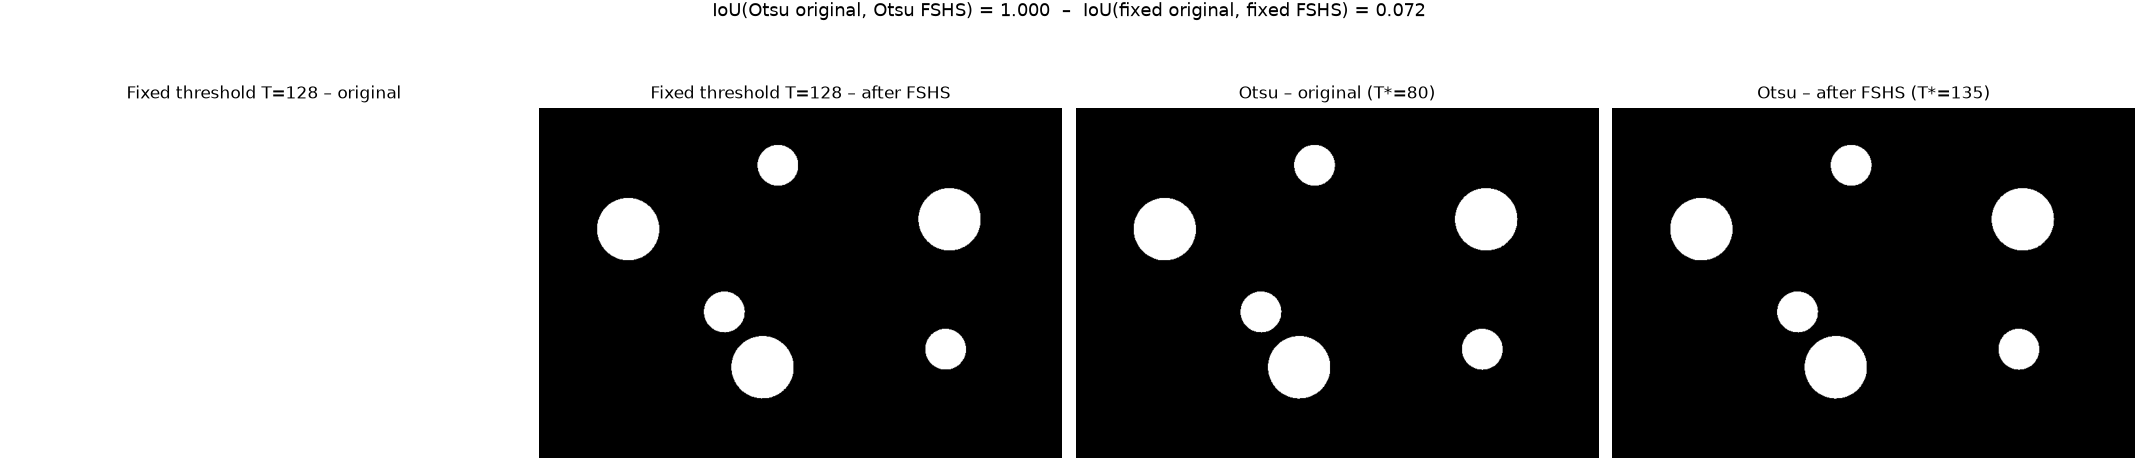
\includegraphics[width=\textwidth]{case2_fshs_threshold.png}
\caption{Case~2: FSHS helps only a \emph{fixed} threshold. With $T=128$ the original image gives an all-foreground mask while the stretched image is segmented correctly (IoU between them $0.072$). With Otsu the threshold moves from $80$ to $135$ but the mask is \emph{identical} (IoU $=1.000$).}
\label{fig:fshs}
\end{figure*}

\begin{figure*}[!t]
\centering
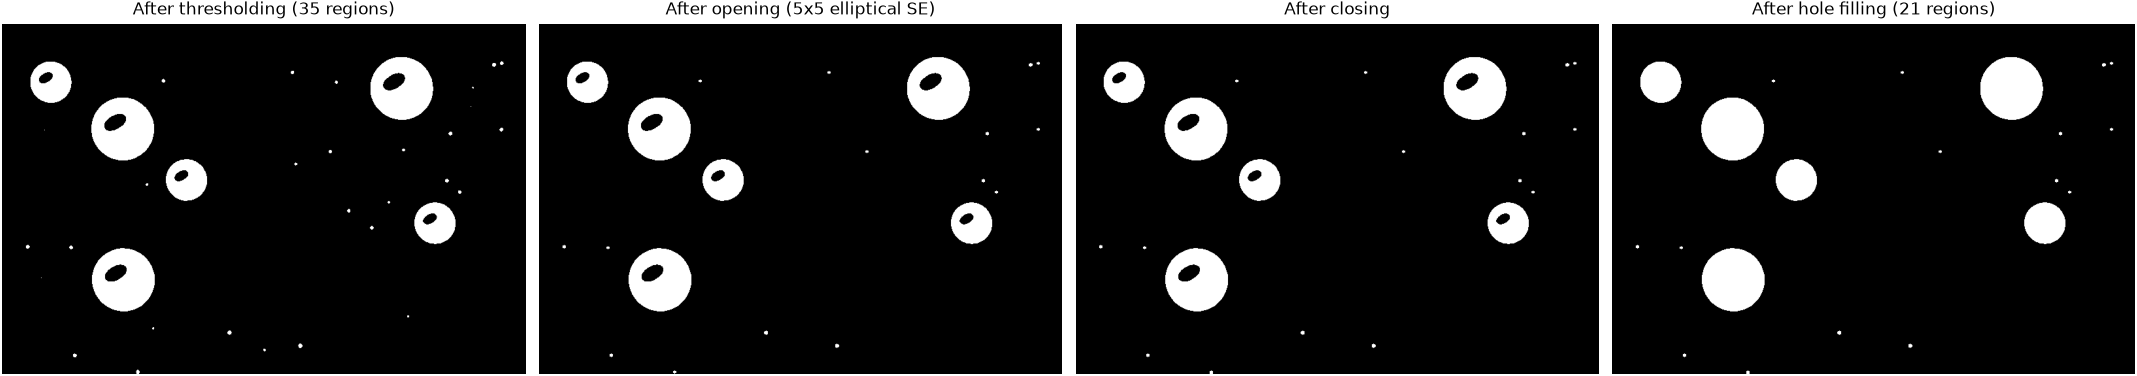
\includegraphics[width=\textwidth]{case3_morphology.png}
\caption{Case~3: mask post-processing. Thresholding gives 35 regions; opening removes small specks; closing seals gaps; hole filling closes glare holes larger than the SE (21 regions). The area filter then removes the remaining dust.}
\label{fig:morph}
\end{figure*}

\begin{figure}[!t]
\centering
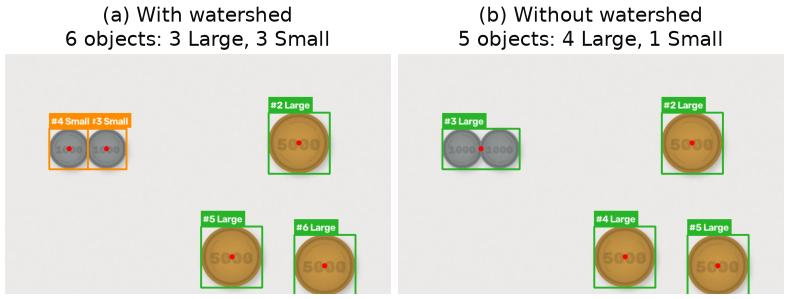
\includegraphics[width=\columnwidth]{case4_split.jpg}
\caption{Case~4: (a) watershed separates the two overlapping small coins; (b) without watershed they merge into one region that is misclassified as a Large coin.}
\label{fig:case4}
\end{figure}

% -----------------------------------------------------------------------------
\subsection{Real Images: Overall Results}
\begin{table*}[!t]
\centering
\caption{Real images (Roboflow~100 \emph{coins}). ``Exact'' and ``$\pm1$'' are the percentages of images counted exactly and within one object. Rows add one module at a time; all choices are based on the \textbf{development} set, and the \textbf{test} set is run only for the main configurations. The highlighted row is the final configuration.}
\label{tab:real}
\footnotesize
\setlength{\tabcolsep}{3pt}
\begin{tabular}{@{}llcccccc@{\hspace{8pt}}ccccc@{}}
\toprule
& & \multicolumn{6}{c}{\textbf{Development} (480 images, 3\,422 coins)} & \multicolumn{5}{c}{\textbf{Test} (480 images, 3\,386 coins)}\\
\cmidrule(lr){3-8}\cmidrule(l){9-13}
& Configuration & Exact & $\pm1$ & MAE & P & R & F1 & Exact & MAE & P & R & F1\\
\midrule
A & Baseline: Otsu on gray & 12.5 & 33.3 & 3.78 & 0.472 & 0.567 & 0.515 & 12.9 & 4.58 & 0.403 & 0.510 & 0.450\\
B & A + illumination flattening & 9.6 & 27.5 & 7.51 & 0.314 & 0.567 & 0.404 & -- & -- & -- & -- & --\\
C & K-Means on gray & 11.9 & 32.7 & 3.75 & 0.483 & 0.585 & 0.529 & 12.1 & 4.51 & 0.412 & 0.528 & 0.463\\
D & Background diff.\ (gray) + Otsu & 23.1 & 47.1 & 5.09 & 0.516 & 0.842 & 0.640 & -- & -- & -- & -- & --\\
F & Background diff.\ (Lab) + Otsu & 22.3 & 46.0 & 5.37 & 0.537 & 0.920 & 0.678 & -- & -- & -- & -- & --\\
G & Background diff.\ (Lab) + Triangle & 9.4 & 17.1 & 9.22 & 0.431 & 0.987 & 0.600 & 7.5 & 8.85 & 0.438 & 0.988 & 0.607\\
I & G + shape filter (circ.\ $\ge0.5$) & 12.5 & 22.9 & 6.84 & 0.502 & 0.981 & 0.664 & -- & -- & -- & -- & --\\
K & I without watershed & 32.7 & 64.8 & 1.48 & 0.821 & 0.928 & 0.871 & -- & -- & -- & -- & --\\
L & I + border clearing & 44.6 & 64.8 & 1.52 & 0.817 & 0.978 & 0.891 & -- & -- & -- & -- & --\\
M & L + gated watershed (circ.\ $\ge0.35$) & 50.0 & 70.4 & 1.17 & 0.863 & 0.968 & 0.912 & -- & -- & -- & -- & --\\
N & M + small-fragment removal & 66.0 & 83.5 & 0.69 & 0.925 & 0.966 & 0.945 & 61.5 & 0.83 & 0.906 & 0.965 & 0.935\\
Q & N with Otsu instead of Triangle & 59.6 & 81.9 & 0.86 & 0.949 & 0.887 & 0.917 & -- & -- & -- & -- & --\\
R & N with gray instead of Lab & 55.0 & 75.8 & 1.02 & 0.867 & 0.910 & 0.888 & -- & -- & -- & -- & --\\
\rowcolor{best} V & N + window $0.15$ + circ.\ $\ge0.6$ (final) & \textbf{70.0} & \textbf{87.9} & \textbf{0.58} & 0.944 & 0.963 & \textbf{0.954} & \textbf{65.4} & \textbf{0.77} & 0.921 & 0.959 & \textbf{0.940}\\
X & V without watershed & 64.4 & 85.4 & 0.64 & 0.975 & 0.926 & 0.950 & 60.8 & 0.77 & 0.959 & 0.921 & 0.939\\
\bottomrule
\end{tabular}
\end{table*}

\begin{figure}[!t]
\centering
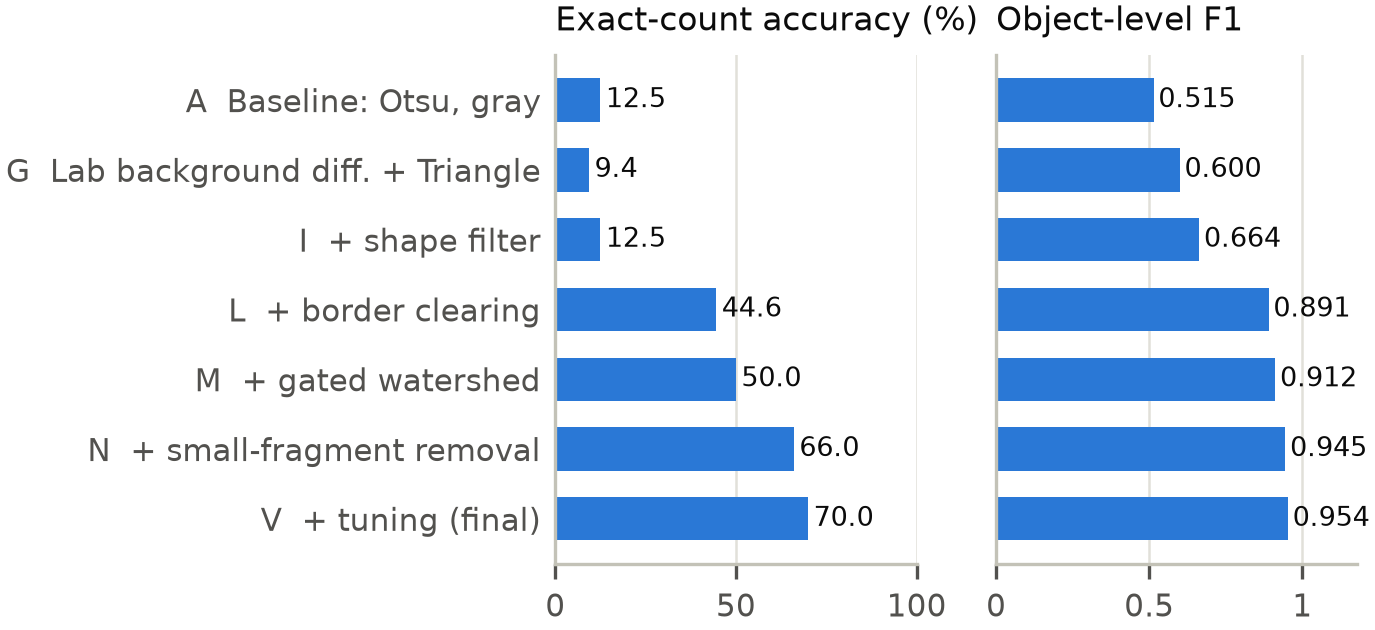
\includegraphics[width=\columnwidth]{chart_ablation.png}
\caption{Cumulative contribution of each module on the development set. Border clearing (L) and small-fragment removal (N) give the largest gains.}
\label{fig:ablation}
\end{figure}

\begin{figure}[!t]
\centering
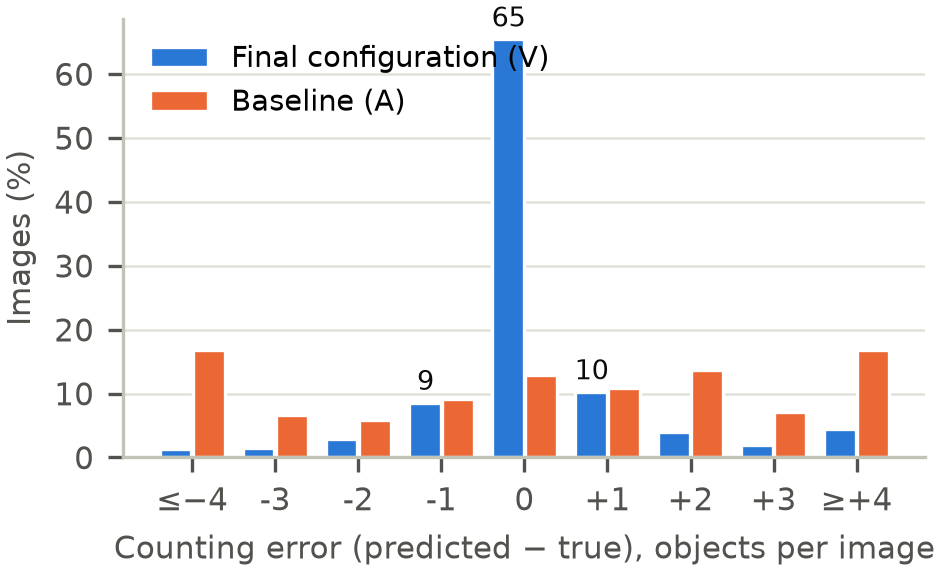
\includegraphics[width=\columnwidth]{chart_count_error.png}
\caption{Distribution of the counting error on the test set. The baseline (A) spreads to both sides; the final configuration (V) concentrates at 0 ($65\%$) and $\pm1$ ($19\%$).}
\label{fig:counterr}
\end{figure}

Table~\ref{tab:real} and Fig.~\ref{fig:ablation} trace the development of the real-image branch:
\begin{itemize}
\item \emph{Background difference} raises recall from $0.567$ (A) to $0.987$ (G): almost no coin is missed. It also produces many false regions (P $=0.431$), so on its own G is even worse than A in exact-count accuracy.
\item \emph{Watershed cuts both ways.} Ungated, it chops table edges into round fragments: disabling it (K) gives F1 $0.871$ versus $0.664$ for I. Once gated by circularity it helps: from X to V, recall rises from $0.926$ to $0.963$ and test exact-count accuracy from $60.8\%$ to $65.4\%$.
\item \emph{Color matters}: using gray (R) instead of Lab (N) lowers exact-count accuracy from $66.0\%$ to $55.0\%$.
\item \emph{Triangle vs.\ Otsu on $D$}: Otsu (Q) is more conservative (P $0.949$) but misses coins (R $0.887$); Triangle with the shape filter (N) is better balanced.
\end{itemize}
On the test set, the final configuration V reaches $65.4\%$ exact-count accuracy, $84.2\%$ within $\pm1$, MAE $0.77$ and F1 $0.940$, against $12.9\%$, $32.9\%$, $4.58$ and $0.450$ for the baseline (Fig.~\ref{fig:counterr}). The test score is slightly below the development score ($65.4\%$ vs.\ $70.0\%$), which is the expected optimism of tuning on the development set and the reason for keeping a separate test set.

% -----------------------------------------------------------------------------
\subsection{Real Images: Results per Case}
\begin{table*}[!t]
\centering
\caption{Test-set results per real case: baseline (A) vs.\ final configuration (V)}
\label{tab:percase}
\footnotesize
\setlength{\tabcolsep}{4pt}
\begin{tabular}{@{}lrr@{\hspace{10pt}}ccc@{\hspace{10pt}}cccccc@{}}
\toprule
& & & \multicolumn{3}{c}{\textbf{Baseline (A)}} & \multicolumn{6}{c}{\textbf{Final (V)}}\\
\cmidrule(lr){4-6}\cmidrule(l){7-12}
Real case & Images & Coins & Exact (\%) & MAE & F1 & Exact (\%) & $\pm1$ (\%) & MAE & P & R & F1\\
\midrule
R1 Ideal & 232 & 1\,745 & 12.9 & 3.03 & 0.676 & \textbf{84.1} & 94.0 & 0.33 & 0.966 & 0.988 & \textbf{0.977}\\
R2 Low contrast & 88 & 599 & 5.7 & 4.82 & 0.181 & \textbf{52.3} & 77.3 & 1.25 & 0.855 & 0.963 & \textbf{0.906}\\
R3 Textured background & 132 & 847 & 19.7 & 7.49 & 0.226 & \textbf{50.8} & 78.0 & 0.98 & 0.894 & 0.943 & \textbf{0.918}\\
R4 Touching coins & 28 & 195 & 3.6 & 2.82 & 0.351 & \textbf{21.4} & 53.6 & 1.96 & 0.865 & 0.754 & \textbf{0.805}\\
\midrule
All & 480 & 3\,386 & 12.9 & 4.58 & 0.450 & \textbf{65.4} & 84.2 & 0.77 & 0.921 & 0.959 & \textbf{0.940}\\
\bottomrule
\end{tabular}
\end{table*}

\begin{figure}[!t]
\centering
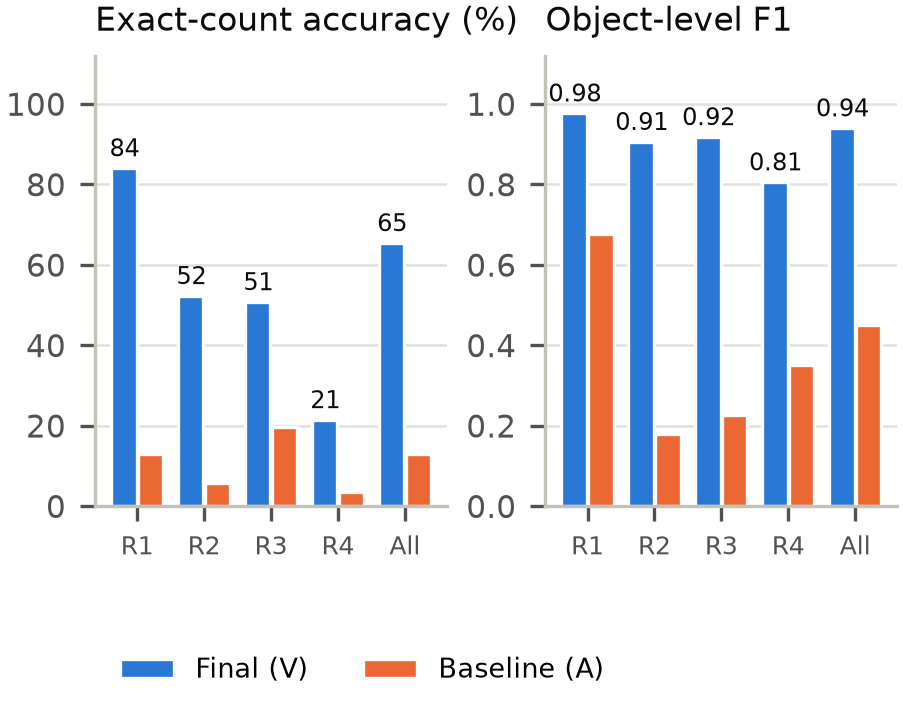
\includegraphics[width=\columnwidth]{chart_real_cases.png}
\caption{Test-set results per real case (R1 ideal, R2 low contrast, R3 textured background, R4 touching coins). The final configuration improves every case; touching coins remain the hardest.}
\label{fig:realcases}
\end{figure}

\begin{figure*}[!t]
\centering
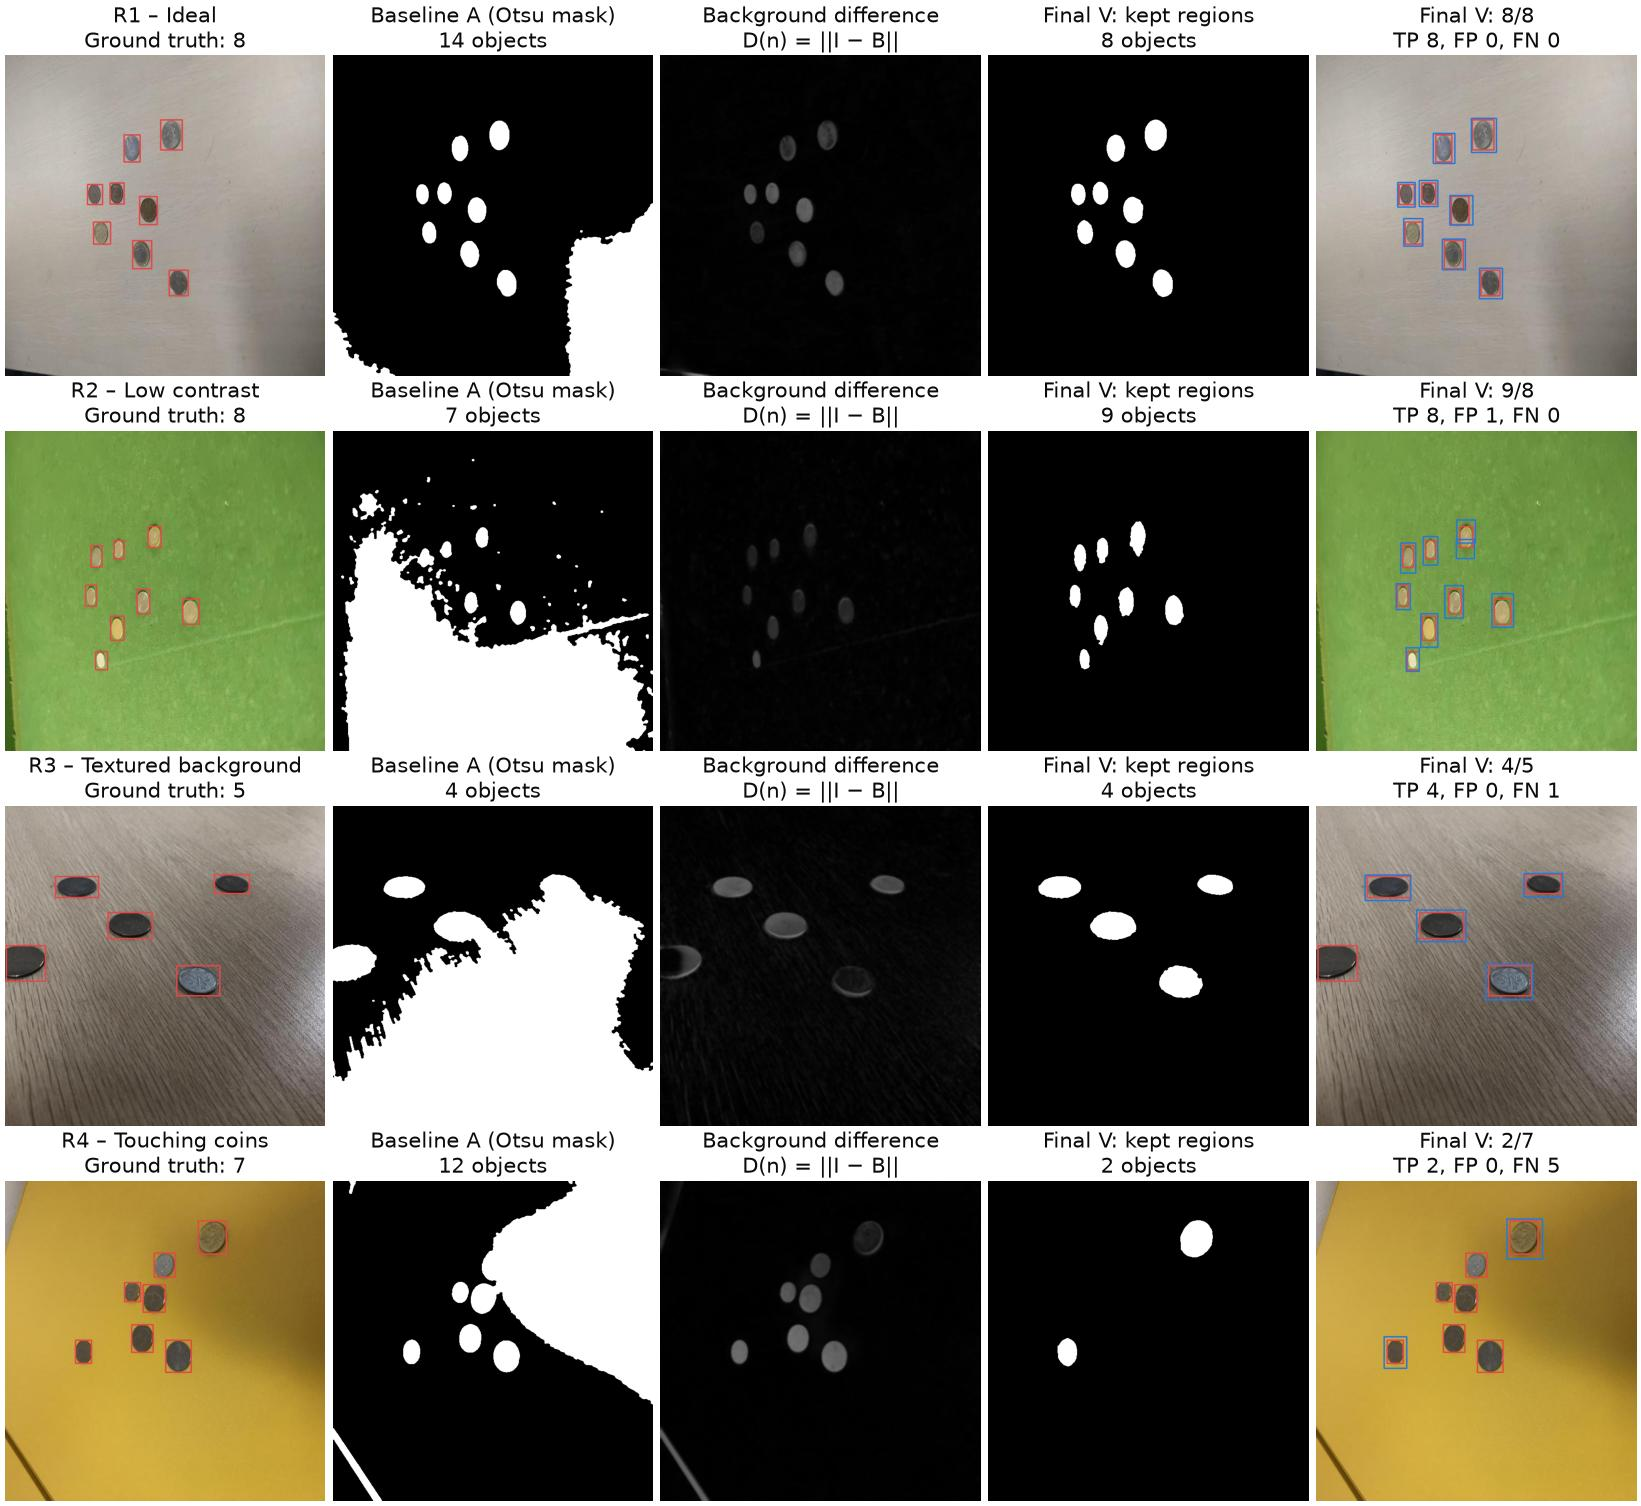
\includegraphics[width=\textwidth]{real_grid.jpg}
\caption{One randomly selected test image (fixed seed) per real case (rows). Columns: input with ground-truth boxes (\textcolor{gtred}{red}); baseline Otsu mask; background-difference image $D(\mathbf{n})$; regions kept by the final configuration; final detections (\textcolor{predblue}{blue}) over the ground truth. The baseline mask is dominated by background shading in every row. Row R4 is a typical failure: the touching coins merge with a shaded background patch into one region of circularity $0.29$, which is neither split (gate $0.35$) nor kept (filter $0.6$), so five coins are lost.}
\label{fig:realgrid}
\end{figure*}

Table~\ref{tab:percase}, Fig.~\ref{fig:realcases} and Fig.~\ref{fig:realgrid} break the test results down by real case:

\textbf{R1 -- Ideal (232 images).} The final configuration counts $84.1\%$ of the images exactly, with F1 $0.977$. Yet the baseline reaches only $12.9\%$: even ``ideal'' photographs contain illumination gradients and table edges, which the global threshold mistakes for objects (Fig.~\ref{fig:realgrid}, row R1). The synthetic Case~1 does not capture this, because its background is perfectly flat.

\textbf{R2 -- Low contrast (88 images).} Exact-count accuracy rises from $5.7\%$ to $52.3\%$ and F1 from $0.181$ to $0.906$. Recall stays high ($0.963$) thanks to the Lab difference image, but precision drops to $0.855$, the lowest of all cases. A likely cause is that the Triangle threshold on $D$ adapts downward when coins differ little from the background, letting more background speckle through.

\textbf{R3 -- Textured background (132 images).} F1 rises from $0.226$ to $0.918$. A typical remaining error is wood grain that touches a coin: the merged region falls below the circularity filter and the coin is lost (Fig.~\ref{fig:realexamples}, \texttt{hf\_0024}).

\textbf{R4 -- Touching coins (28 images).} This is the hardest case: $21.4\%$ exact-count accuracy and recall $0.754$. The synthetic Case~4 contained one pair of equal coins on a clean background; real clusters contain three or more coins and often merge with shadows (Fig.~\ref{fig:realgrid}, row R4), which defeats both the watershed and the shape filter.

\begin{figure*}[!t]
\centering
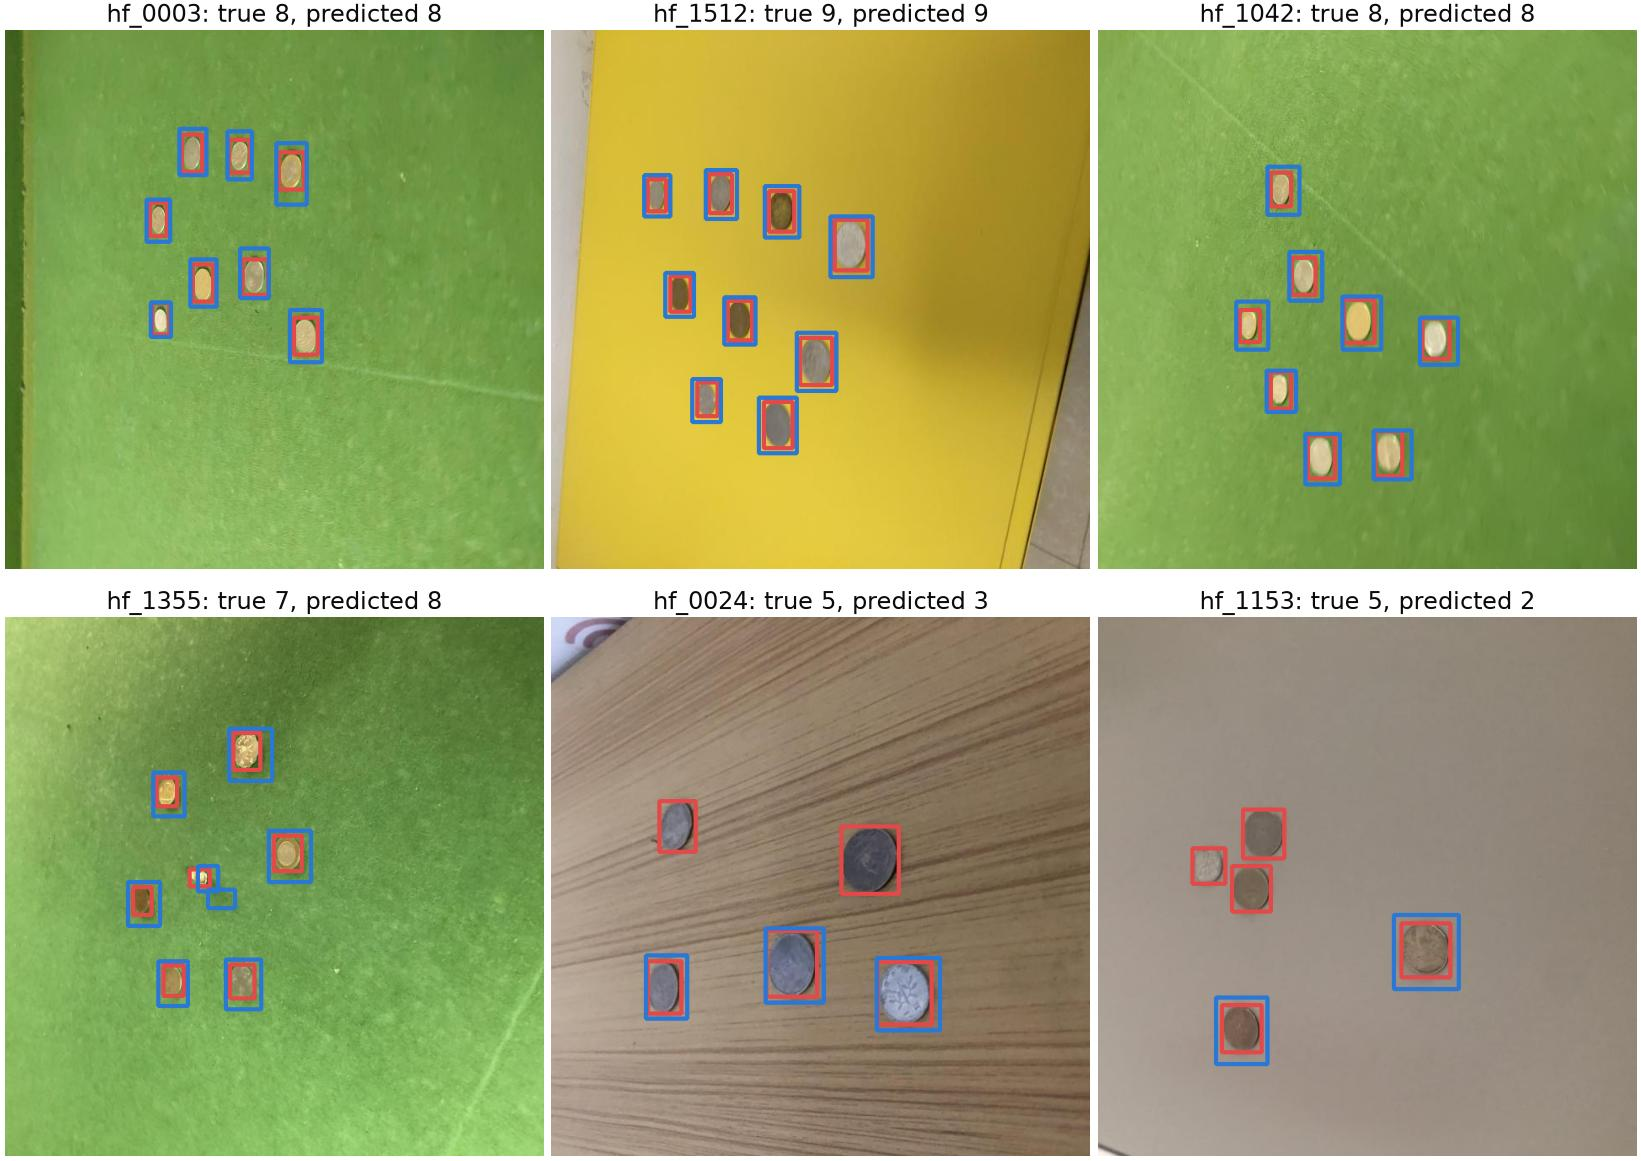
\includegraphics[width=\textwidth]{real_examples.jpg}
\caption{Test examples (\textcolor{gtred}{red}: ground truth, \textcolor{predblue}{blue}: prediction). Top row: correct counts on green mats and yellow paper. Bottom row: typical errors. \texttt{hf\_1355}: a small coin with its shadow is split in two. \texttt{hf\_0024}: wood grain attached to the coin edges pushes circularity below $0.6$ and the coins are removed. \texttt{hf\_1153}: a cluster of three touching coins is not separated.}
\label{fig:realexamples}
\end{figure*}

% -----------------------------------------------------------------------------
\subsection{Run Time}\label{sec:timing}
\begin{figure}[!t]
\centering
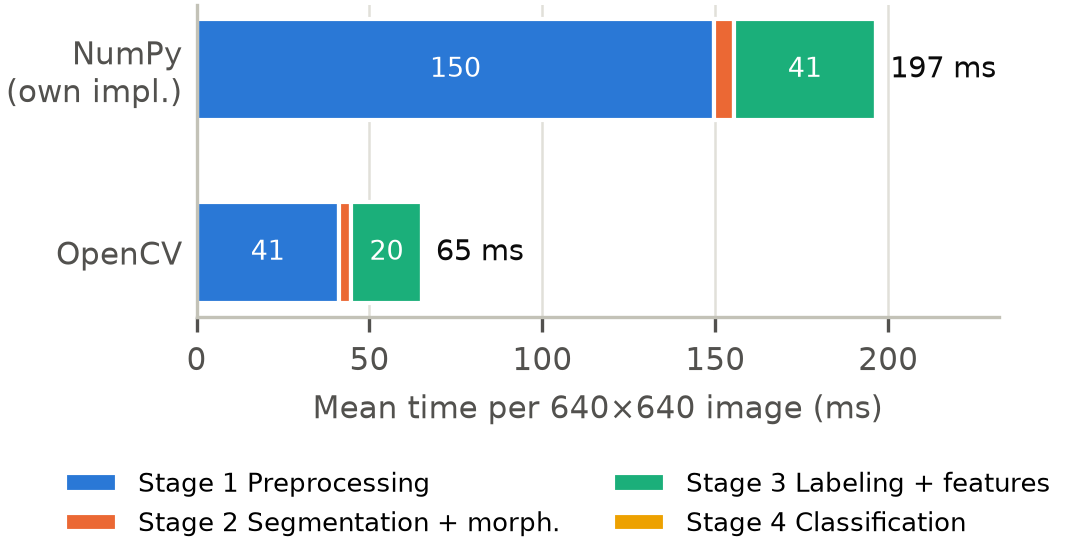
\includegraphics[width=\columnwidth]{chart_timing.png}
\caption{Mean time per stage for configuration V (100 test images, single thread). Stage~4 takes under $0.1$\,ms and is not visible.}
\label{fig:timing}
\end{figure}
Fig.~\ref{fig:timing} shows that configuration V takes on average $65$\,ms per image with the OpenCV backend and $197$\,ms with our own implementation, excluding image decoding. Most of the time is spent in Stage~1 (median filtering and background estimation); our NumPy median filter is about 200 times slower than OpenCV's (Table~\ref{tab:verify}). On the first 60 test images both backends give the same F1 ($0.921$), so the two backends differ in speed only, not in accuracy.

% =============================================================================
\section{Discussion}\label{sec:discussion}
% =============================================================================
\textbf{From synthetic to real cases.} The four synthetic cases each isolate one difficulty, and on them the pipeline is perfect. The real cases contain the same difficulties in a harder form. R1 shows that a real ``ideal'' scene is less ideal than Case~1, because of illumination gradients. In R2, low contrast is local and chromatic rather than global, so FSHS cannot help but color can. In R3, noise is structured (grain lines) rather than isolated specks. In R4, real touching groups are larger and shadowed. Synthetic tests are therefore necessary to validate each module, but not sufficient to predict real-world accuracy.

\textbf{FSHS and Otsu.} If $g=af+b$ with $a>0$, a threshold $t$ on $f$ corresponds to the threshold $at+b$ on $g$ and produces the same two classes, while $\sigma_b^2$ in~\eqref{eq:otsu} is simply multiplied by $a^2$. Hence, apart from rounding and the few pixels clipped at the percentiles, Otsu on the stretched image returns \emph{the same mask} as on the original. The same argument applies to one-dimensional K-Means. Fig.~\ref{fig:fshs} confirms this experimentally (IoU $=1.000$). The original specification's claim that FSHS ``helps Otsu separate the background'' is therefore incorrect: FSHS only helps fixed thresholds and visualization.

\textbf{Otsu and K-Means.} Two-cluster K-Means on gray levels converges to $T=(\mu_0+\mu_1)/2$, the fixed point of the Ridler--Calvard iteration~\cite{ridler1978}. This is a stationary point of Otsu's criterion, not necessarily its global maximum, but usually very close to it. On synthetic images the two thresholds coincide; on real images the results differ slightly ($12.5\%$ vs.\ $11.9\%$ on the development set).

\textbf{A correct count is not a correct segmentation.} Counting accuracy alone can hide errors: a merged blob plus a spurious fragment still yields the right number. This is why we always report mask IoU (synthetic) and object-level P/R/F1 (real) in addition to counts.

\textbf{Why the baseline fails on real images.} Coins cover $2.1\%$ of the image on average (90th percentile: $3.0\%$). With such a small class weight $\omega_1$, Otsu's between-class variance is maximized by contrasts \emph{within the background} (bright/dark areas, table edges). Illumination flattening (B) does not help either, because real backgrounds have structure (edges, grain) rather than only slowly varying illumination.

\textbf{Limitations.} (i) The real data have no size labels, so Large/Small classification is validated only on synthetic images; self-captured photographs with size labels are needed. (ii) The publisher's $640\times640$ resizing stretches coins into ellipses; the circularity threshold of $0.6$ accounts for this. (iii) The real-branch parameters were selected for this dataset; other backgrounds or object sizes require re-selection on a new development set. (iv) R4 contains only 28 test images, so its estimate is less certain than the others. (v) We did not train a deep detector for a direct comparison. Detectors such as YOLO~\cite{redmon2016} would likely handle grain, shadows and clusters better, at the cost of labeled data and GPU training.

% =============================================================================
\section{Conclusion and Future Work}
% =============================================================================
We built and quantitatively evaluated a classical pipeline for counting and size-classifying objects. On four controlled synthetic cases, each module behaves as theory predicts and every object is counted and classified correctly. On four real-image cases drawn from 960 photographs, the ``uniform background'' and ``bimodal histogram'' assumptions break down, and the baseline counts only $12.9\%$ of the test images exactly. A real-image branch based on color background subtraction, Triangle thresholding and shape constraints raises this to $65.4\%$ (F1 $0.940$; from $0.977$ on ideal scenes to $0.805$ on touching coins), still without any training and at about $65$\,ms per image on a CPU.

\textbf{Future work:} (1) collect self-captured images with size labels to evaluate classification on real data; (2) seed the watershed with H-maxima to separate clusters of three or more coins; (3) use locally adaptive thresholds or Gaussian mixture models for structured backgrounds; (4) extend the system to video with frame-to-frame change detection and object tracking; (5) compare directly with a deep detector trained on the Roboflow~100 \emph{coins} training split.

% =============================================================================
\appendices
\section{Course Content and Source Modules}
\begin{table}[!h]
\centering
\caption{IMP302m chapters and the corresponding implementation modules}
\label{tab:mapping}
\footnotesize
\setlength{\tabcolsep}{3pt}
\begin{tabular}{@{}p{1.75cm}p{3.75cm}p{2.4cm}@{}}
\toprule
Chapter & Technique & Module\\
\midrule
Ch.~1.1 & Histogram, AOD, FSHS, NN interpolation & \cfg{preprocess.py}\\
Ch.~1.2 & Otsu, region labeling, binary morphology & \cfg{segmentation.py}, \cfg{labeling.py}, \cfg{morphology.py}\\
Ch.~2, 3 & Gaussian and median filtering; degradation model & \cfg{preprocess.py}\\
Ch.~7, 8 & Sampling and quantization & \cfg{preprocess.py}\\
Ch.~9.1 & K-Means clustering & \cfg{segmentation.py}\\
Ch.~9 & Watershed (touching objects) & \cfg{split.py}\\
Ch.~9.5 & Change detection $\rightarrow$ background difference & \cfg{preprocess.py}\\
Ch.~10 & Area, perimeter, diameter, circularity & \cfg{features.py}\\
Ch.~11.1 & Contours and bounding boxes & \cfg{features.py}\\
Ch.~12 & Rule-based pattern classification & \cfg{classify.py}\\
\bottomrule
\end{tabular}
\end{table}

% =============================================================================
\begin{thebibliography}{99}
\bibitem{bovik2005handbook}
A.~C. Bovik, Ed., \emph{Handbook of Image and Video Processing}, 2nd~ed. Burlington, MA, USA: Academic Press, 2005.

\bibitem{gonzalez2018dip}
R.~C. Gonzalez and R.~E. Woods, \emph{Digital Image Processing}, 4th~ed. New York, NY, USA: Pearson, 2018.

\bibitem{otsu1979}
N.~Otsu, ``A threshold selection method from gray-level histograms,'' \emph{IEEE Trans. Syst., Man, Cybern.}, vol.~9, no.~1, pp.~62--66, 1979.

\bibitem{ridler1978}
T.~W. Ridler and S.~Calvard, ``Picture thresholding using an iterative selection method,'' \emph{IEEE Trans. Syst., Man, Cybern.}, vol.~8, no.~8, pp.~630--632, 1978.

\bibitem{macqueen1967}
J.~MacQueen, ``Some methods for classification and analysis of multivariate observations,'' in \emph{Proc. 5th Berkeley Symp. Math. Statist. Probab.}, 1967, pp.~281--297.

\bibitem{zack1977}
G.~W. Zack, W.~E. Rogers, and S.~A. Latt, ``Automatic measurement of sister chromatid exchange frequency,'' \emph{J. Histochem. Cytochem.}, vol.~25, no.~7, pp.~741--753, 1977.

\bibitem{sezgin2004}
M.~Sezgin and B.~Sankur, ``Survey over image thresholding techniques and quantitative performance evaluation,'' \emph{J. Electron. Imaging}, vol.~13, no.~1, pp.~146--165, 2004.

\bibitem{serra1982}
J.~Serra, \emph{Image Analysis and Mathematical Morphology}. London, U.K.: Academic Press, 1982.

\bibitem{rosenfeld1966}
A.~Rosenfeld and J.~L. Pfaltz, ``Sequential operations in digital picture processing,'' \emph{J. ACM}, vol.~13, no.~4, pp.~471--494, 1966.

\bibitem{vincent1991}
L.~Vincent and P.~Soille, ``Watersheds in digital spaces: An efficient algorithm based on immersion simulations,'' \emph{IEEE Trans. Pattern Anal. Mach. Intell.}, vol.~13, no.~6, pp.~583--598, 1991.

\bibitem{meyer1994}
F.~Meyer, ``Topographic distance and watershed lines,'' \emph{Signal Process.}, vol.~38, no.~1, pp.~113--125, 1994.

\bibitem{radke2005}
R.~J. Radke, S.~Andra, O.~Al-Kofahi, and B.~Roysam, ``Image change detection algorithms: A systematic survey,'' \emph{IEEE Trans. Image Process.}, vol.~14, no.~3, pp.~294--307, 2005.

\bibitem{ren2015}
S.~Ren, K.~He, R.~Girshick, and J.~Sun, ``Faster R-CNN: Towards real-time object detection with region proposal networks,'' in \emph{Proc. NeurIPS}, 2015, pp.~91--99.

\bibitem{redmon2016}
J.~Redmon, S.~Divvala, R.~Girshick, and A.~Farhadi, ``You only look once: Unified, real-time object detection,'' in \emph{Proc. IEEE CVPR}, 2016, pp.~779--788.

\bibitem{carion2020}
N.~Carion, F.~Massa, G.~Synnaeve, N.~Usunier, A.~Kirillov, and S.~Zagoruyko, ``End-to-end object detection with transformers,'' in \emph{Proc. ECCV}, 2020, pp.~213--229.

\bibitem{dosovitskiy2021}
A.~Dosovitskiy \emph{et~al.}, ``An image is worth 16x16 words: Transformers for image recognition at scale,'' in \emph{Proc. ICLR}, 2021.

\bibitem{ciaglia2022rf100}
F.~Ciaglia, F.~S. Zuppichini, P.~Guerrie, M.~McQuade, and J.~Solawetz, ``Roboflow 100: A rich, multi-domain object detection benchmark,'' \emph{arXiv preprint arXiv:2211.13523}, 2022. Dataset: \url{https://universe.roboflow.com/object-detection/coins-1apki}

\bibitem{bradski2000opencv}
G.~Bradski, ``The OpenCV library,'' \emph{Dr. Dobb's J. Softw. Tools}, 2000.

\bibitem{vanderwalt2014}
S.~van~der Walt \emph{et~al.}, ``scikit-image: Image processing in Python,'' \emph{PeerJ}, vol.~2, p.~e453, 2014.

\bibitem{harris2020numpy}
C.~R. Harris \emph{et~al.}, ``Array programming with NumPy,'' \emph{Nature}, vol.~585, pp.~357--362, 2020.
\end{thebibliography}

\end{document}
